% The following defines de document class plus some options:
% 12pto: Size of the font
% a4paper: Size of sheet
% twoside: Printable in both sides
% openright: Chapters open in right-hand page
% titlepage: Causes the \maketitle command to make a separate title page and the abstract environment to put the abstract on a separate page. 
% fleqn: Left-aligns displayed formulas
\documentclass[11pt,a4paper,twoside,openright,titlepage,fleqn]{book}

% Extra packages and options
%=============================================================================PACKAGES=========================================================================================
% Allows to change several parameters from headers and footers
\usepackage{fancyhdr}

% Allows to change space between lines
\usepackage{setspace}          

% Allows tables to occupy several pages
\usepackage{longtable}         

% Landscape command is in the following package
\usepackage{lscape} 

% Packet geometry to design document
\usepackage[left=2.5cm,right=2.5cm,top=2.5cm,bottom=2.5cm,footskip=1cm]{geometry}
\parindent = 5mm		% Sangría

% fixltx2e allows for the use of subscripts and superscripts inside the text
\usepackage{fixltx2e}           

% Commands relative to color
% color: Package to use color
% usenames, dvipsnames and svgnames give access to a lot of colors
% table is for including color in tables
\usepackage[usenames,dvipsnames,svgnames,table]{xcolor}

% Package to change color to references (taken from: http://tex.stackexchange.com/questions/197293/change-the-color-of-cite-number-in-bibliography)
\usepackage{xpatch}

% Allows to rotate PSs and EPSs
\usepackage{rotating}          

% Euro symbol
\usepackage{textcomp}          %

% Allows to include several TOC in every chapter
%\usepackage[spanish]{minitoc}           
\usepackage{titletoc}

% Manipulations for EPSs
\usepackage{epsf}            

% This is useful for the frontpage (arbitrary text positioning)
\usepackage[absolute]{textpos} 

% Spanish support and encondig (two following packages)
\usepackage[main=spanish, english]{babel}   
\usepackage[utf8]{inputenc} 

% Standard package for selecting font encodings
\usepackage[T1]{fontenc}

% Fonts to typeset mathematics to match Palatino
\usepackage{mathpazo}		% Defines Mathpatho font
\linespread{1.05}         	% Palatino needs more leading (space between lines)

% makeidx creates an index
\usepackage{makeidx}

% nomencl creates a nomenclature
% intoc: Puts the nomenclature in the TOC
% spanish: For Spanish Language
\usepackage[intoc,spanish]{nomencl}
% glossaries is more up to date than nomencl
%\usepackage[xindy,nonumberlist,toc,nopostdot,style=altlist,nogroupskip]{glossaries}

% Graphics inclusion, support for \figure (see below)
\usepackage{graphicx} 

% subfig package allows for sub-floats (figures, tables) to be separately captioned, referenced and included in a list-of-floats page
\usepackage{subfig}

% For the bibliography (natbib allows for multiple bibliographies in one document)
\usepackage[sort&compress,super,comma, square, sectionbib]{natbib}
\usepackage{chapterbib}

% Integrating notes into the bibliography
\usepackage{notes2bib}

% Enhanced multiple citations
\usepackage{mciteplus}

% cite package allows as to manipulate how cites are formed. This package is not compatible with biblatex
\usepackage{cite}

% Use aditional symbols (AMS)
\usepackage{amsmath,amssymb,amsfonts,latexsym}

% Extension of the keyval package
\usepackage{xkeyval}

% Enumerate with redefinable labels
\usepackage{enumerate}

% lettrine used capital letter
\usepackage{lettrine}

% Define the name of Tables
\usepackage[format=plain,justification=centerlast,width=15cm,labelsep=period,tablename=Tabla,skip=5pt]{caption}

% appendix allows for more control over the appendixes format
\usepackage{appendix}

% Add bibliography/index/contents to Table of Contents
\usepackage[nottoc]{tocbibind}

% Package for backreferencing
\usepackage[ref]{backref}

% hyperref is used for hyperlinks
% colorlinks: To show links with color
% linkcolor = color: Color of links
% urlcolor = color: Color of url links
% citecolor = color: Color of bibliographic references
% linktoc = all: For numbers in TOC colored as well
% backref = For backreferencing the citations in the global bibliography
\usepackage[linktoc=all,backref=section]{hyperref}
% Change hyperref behaviour
\hypersetup{
	colorlinks=true,
	citecolor=violet,
	linkcolor=red,
	urlcolor=blue,
	citebordercolor=violet,
	filebordercolor=red,
	linkbordercolor=blue}

% lastpage package allows for the use of the lastpage
\usepackage{lastpage}

% Titleref provides a command \titleref to cross-reference the titles of sections
\usepackage{titleref}

% backref package allows for backreferencing citations in the bibliography when used in per chapter bibliography
% ref: section number for reference. This package is not compatible with biblatex
%\usepackage[ref]{backref}

% Multirow package allows for the creation of tables
\usepackage{multirow}

% enumitem package allows the changing of enumeration style (roman numbers...)
\usepackage{enumitem}

% Define the name of Tables
\usepackage[format=plain,justification=centerlast,width=15cm,labelsep=period,tablename=Tabla,skip=5pt]{caption}

% Multiple columns (for index)
\usepackage{multicol}

%=============================================================================================================================================================================

% Softens the line breaking rules from LaTeX
\sloppy 

% Changes decimal symbol to a point
\spanishdecimal{.}		

% To use normal spacing after '.'
\frenchspacing 

% The following commands allow the subsubsubsection to be numbered in the text and in the index
\setcounter{secnumdepth}{4}		% For the text
\setcounter{tocdepth}{4}		% For the index


% Basic header and footer
\pagestyle{headings} 

% Margin settings
%\setlength{\oddsidemargin}{0pt}     % Left margin for odd pages default 40pt
%\setlength{\evensidemargin}{0pt}    % Left margin even pages default 10pt
%\setlength{\textwidth}{450pt}       % Width of the body (default 400 pt)

%
% Recomendation to enhance the figures location
% (taken from http://dcwww.camp.dtu.dk/~schiotz/comp/LatexTips/LatexTips.html#captfont)
%
\renewcommand{\topfraction}{0.85}
\renewcommand{\textfraction}{0.1}
\renewcommand{\floatpagefraction}{0.75}

% To avoid Unicode char \u9: not set up for use with LaTeX error (taken from: http://tex.stackexchange.com/questions/83440/inputenc-error-unicode-char-u8-not-set-up-for-use-with-latex)
\DeclareUnicodeCharacter{00A0}{ }

% Rename Tables to Tablas in Spanish
\addto\captionsspanish{\renewcommand*{\tablename}{Tabla}}

% Formating for letters and numbers for crossreferences taken from a sublist
\renewcommand{\mcitesubrefform}{$^{\arabic{mcitebibitemcount}\alph{mcitesubitemcount}}$} 
%\providecommand{\mcitesubrefform}{\arabic{mcitebibitemcount}.\alph{mcitesubitemcount}}

% Remove "General Index" from the minitoc
%\renewcommand{\mtctitle}{}

% Spacing from the upper border and where the main text body begins. LaTeX  complains if we use fanchyhdr and headheight is less than 15pt
%
%\headheight 28pt

%
% For textpos package (used for frontpage)
%
\setlength{\TPHorizModule}{\paperwidth}
\setlength{\TPVertModule}{\paperheight}
\newcommand{\tb}[4]{\begin{textblock}{#1}[0.5,0.5](#2,#3)\begin{center}#4\end{center}\end{textblock}}

%
% Command redefinition.
% 
% \newcommand{cmd}[args]{def}
%
% cmd  = command to be redefined (i.e. \char)
% args = number of arguments
% def  = definition, substituting #1, #2... por el first, second... argument
%
% For example:
%
% \newcommand{\water}[1]{H\ensuremath{_#1}O}
%
% Anytime we write "\water{33}", as output would yield: "H33O" (33 as subscript)
%

% Rename Nomenclature
\renewcommand{\nomname}{Lista de Símbolos}

% To change color to cite references in the References Section (not in the main text taken from: http://tex.stackexchange.com/questions/197293/change-the-color-of-cite-number-in-bibliography)
\makeatletter
\xpatchcmd{\@lbibitem}
{\item[\hfil}
{\item[\hfil\color{blue}}
{}{}
\makeatother

% Rename Command in backref so the sections are in brackets
\renewcommand*{\backref}[1]{[#1]}
% Define Spanish words for backreferencing
\def\backrefspanish{%
	\def\backrefpagesname{páginas}%
	\def\backrefsectionsname{secciones}%
	\def\backrefsep{, }
	\def\backreftwosep{ y~}%
	\def\backreflastsep{ y~}%
}

% First pages with Roman numbers
% Later they will be changed to Arabic
%
\pagenumbering{Roman}

% To print nomenclature
\makeglossary
\makenomenclature

% To print index
\makeindex

% The following commands allow the subsubsubsection to be numbered in the text and in the index
\setcounter{secnumdepth}{4}		% For the text
\setcounter{tocdepth}{4}		% For the index

% -----------------------------------------------------------------------------------------------------------------------------------------------
% CODE ZONE
% -----------------------------------------------------------------------------------------------------------------------------------------------
% This code forbids the inserted pages to have either header or footer
\makeatletter
  \def\cleardoublepage{\clearpage\if@twoside \ifodd\c@page\else
  \vspace*{\fill}
    \thispagestyle{empty}
    \newpage
    \if@twocolumn\hbox{}\newpage\fi\fi\fi}
\makeatother


% This code lets the index to be printed in different number of columns (taken from: http://latex-community.org/forum/viewtopic.php?f=4&t=1735)
%\makeatletter
%\renewenvironment{theindex}
%{\if@twocolumn
%	\@restonecolfalse
%	\else
%	\@restonecoltrue
%	\fi
%	\setlength{\columnseprule}{0.5pt}
%	\setlength{\columnsep}{35pt}
%	\begin{multicols}{2}[\section*{\indexname}]
%		\markboth{\MakeUppercase\indexname}%
%		{\MakeUppercase\indexname}%
%		\thispagestyle{plain}
%		\setlength{\parindent}{0pt}
%		\setlength{\parskip}{0pt plus 0.3pt}
%		\relax
%		\let\item\@idxitem}%
%	{\end{multicols}\if@restonecol\onecolumn\else\clearpage\fi}
%\makeatother
\makeatletter
\renewenvironment{theindex}
{\if@twocolumn
	\@restonecolfalse
	\else
	\@restonecoltrue
	\fi
	\setlength{\columnseprule}{0pt}
	\setlength{\columnsep}{35pt}
	\begin{multicols}{2}[\chapter*{\indexname}]          %Adjust the 2 for more columns
		\markboth{\MakeUppercase\indexname}%
		{\MakeUppercase\indexname}%
		\thispagestyle{plain}
		\setlength{\parindent}{0pt}
		\setlength{\parskip}{0pt plus 0.3pt}
		\relax
		\let\item\@idxitem}%
	{\end{multicols}\if@restonecol\onecolumn\else\clearpage\fi}
\makeatother

% This code also puts the first entries in bold
%\makeatletter
%\renewcommand\@idxitem{\scriptsize\bfseries\par\hangindent %40\p@}                       %Makes all the index entries small,  bold
%\renewcommand\subitem{\scriptsize\@idxitem %\normalfont\hspace*{20\p@}}                  %Makes subitems small, normal
%\renewcommand\subsubitem{\scriptsize\@idxitem %\normalfont\hspace*{30\p@}}               %Makes subsubitems small, normal
%\makeatother

% Begin of document
\begin{document}
	\begin{onehalfspace}
	\frontmatter
		%
		% The values of several variables like author, thesis title... are written in rename.tex
		%
		% This file includes some internal variable names

% Solve some issues with babel package in book
\renewcommand{\contentsname}{Contenido}
\renewcommand{\partname}{Parte}
\renewcommand{\appendixname}{Apéndice}
\renewcommand{\figurename}{Figura}
\renewcommand{\listtablename}{Índice de Tablas}
\renewcommand\listfigurename{Índice de Figuras}
\renewcommand{\chaptername}{Capítulo}
\renewcommand{\bibname}{Referencias}
\renewcommand\citeform[1]{(#1)}			% Changes reference format to [(1),(2),(3)]
\renewcommand{\nomname}{Lista de Símbolos}

% Fine tuning to style file. Babel package doesn't correctly produce output for these items:
\addto\captionsspanish{\renewcommand\listtablename{Índice de Tablas}}
\addto\captionsspanish{\renewcommand\listfigurename{Índice de Figuras}}

% Thesis author name
\newcommand{\myname}{Juan José Expósito González}
% Director/s of Thesis
\newcommand{\myboss}{{Magín Lapuerta Amigo}{Francisco J. Martos Ramos}}
%Thesis title
\newcommand{\thesistitle}{Thesis Title}
% Thesis subtitle
\newcommand{\thesissubtitle}{Here it goes!} 
\newcommand{\worktype}{Tesis Doctoral}     
\newcommand{\logo}{Figuras/Escudo.pdf} 
\newcommand{\logodos}{Figuras/EscudoUCLM.png}

% More customization on headers and footers (lowercase and no chapter numbers)
%\renewcommand{\chaptermark}[1]{ \markboth{#1}{} }
%\renewcommand{\sectionmark}[1]{ \markright{#1}{} }

% Define directories where to find figures
\graphicspath{{Figuras/}}

\makeatletter
\renewcommand\@cite[2]{%
	Ref.~#1\ifthenelse{\boolean{@tempswa}}
	{, \nolinebreak[3] #2}{}
}
\renewcommand\@biblabel[1]{[#1]}
\renewcommand{\@cite}[1]{\cite{{#1}}}
\renewcommand\citeform[1]{\textbf{[#1]}}
\renewcommand\citeleft{[} 
\renewcommand\citeright{]} 
\makeatother

\let\cite=\citen


		
		%
		% Preliminar CONTENT: frontpage, certificate, acknowledgments, cites, prefaces...
		%
		\pagestyle{empty}
\begin{figure}[h]
\centering

\includegraphics[scale=0.9]{EscudoUCLM.png}\\
\end{figure}

\begin{center}
\Large{\textbf{UNIVERSIDAD DE CASTILLA-LA MANCHA}}\\
\vspace{0.2cm}
\Large{\textbf{ESCUELA T�CNICA SUPERIOR DE INGENIEROS INDUSTRIALES}}\\
\vspace{0.2cm}
\large{CIUDAD REAL}\\
\vspace{0.2cm}
\Large{TESIS DOCTORAL}\\
\vspace{0.2cm}
\rule[0.3cm]{15cm}{0.1cm}
\Large{\textbf{Estudio de la morfolog�a de las part�culas Di�sel mediante an�lisis fractal}}\\
\end{center}

\begin{table}[h]
	\centering
	\begin{tabular}{ p{ 6cm } p{ 6cm } }
		\begin{center}
			
\includegraphics[width=5cm]{EscudoIndustriales.png}			
		\end{center} &
		\begin{center}
			\large{PRESENTADA POR:}\\
			\vspace{0.5cm}
			\Large{Juan Jos� Exp�sito Gonz�lez}\\
			\vspace{1cm}
			\large{DIRIGIDA POR:}\\
			\vspace{0.5cm}
			D. Mag�n Lapuerta Amigo \\
			D. Francisco Jos� Martos Ramos
		\end{center}
	\end{tabular}
\end{table}

\clearpage
		
		% CONFIG Frontmatter
		% Uses \cdpchapter for all chapters beginning "to the right"
% and lack of number (i.e. Acknoledgments):
\newcommand{\cdpchapter}[1]{\cleardoublepage\chapter*{#1}}

% Begins numbering again:
\setcounter{page}{1}


		
%		\pagestyle{empty}
\section*{Agradecimientos}
\lettrine[lraise=0.1, nindent=0em, slope=-.5em]{R}{edactar} una Tesis es un proceso largo y laborioso. A veces uno desespera y quiere abandonar, porque este camino que hoy termina (o comienza, según se mire) se me ha hecho largo. Largo en el tiempo, largo por 

\cleardoublepage
		\pagestyle{empty}
\begin{center}
\scalebox{0.20}{
\includegraphics{Escudo.pdf}}
\end{center}
\begin{center}
\vspace{0.5cm}
{\large UNIVERSIDAD DE CASTILLA-LA MANCHA}\\ \vspace{0.2cm}
{\large DEPARTAMENTO DE MECÁNICA APLICADA E INGENIERÍA DE PROYECTOS}\\ \vspace{0.2cm}
{\large ESCUELA TÉCNICA SUPERIOR DE INGENIEROS INDUSTRIALES}\\ \vspace{0.2cm}
\rule{\linewidth}{1.5pt}\\
\vspace{0.5cm}
\renewcommand{\baselinestretch}{2.0}
\large\normalsize
{\huge Estudio de la morfología de las partículas Diésel mediante análisis fractal}\\
\vspace{3.0cm}
\renewcommand{\baselinestretch}{1.0}
\large\normalsize
{\Large TESIS DOCTORAL}\\ \vspace{2.5cm}
{\Large PRESENTADA POR:}\\ \vspace{0.2cm}
{\Large Juan José Expósito González}\\ \vspace{0.8cm}
{\Large DIRIGIDA POR:}\\ \vspace{0.2cm}
{\Large Dr. D. Magín Lapuerta Amigo}\\ \vspace{0.2cm}
{\Large Dr. D. Francisco José Martos Ramos}\\ \vspace{1.5cm}
{\Large Ciudad Real, 201X}\\ \vspace{1.5cm}
\end{center}

\clearpage
		\pagestyle{empty}
\vspace*{2cm}
\begin{center}
{\large TESIS DOCTORAL}\\
\vspace{1.5cm}
{\huge Estudio de la morfolog�a de las part�culas Di�sel mediante an�lisis fractal}\\
\vspace{2.5cm}
\renewcommand{\baselinestretch}{2.0}
PRESENTADA POR:\\
{\large Juan Jos� Exp�sito Gonz�lez}\\ \vspace{1.0cm}
DIRIGIDA POR:\\
{\large Dr. D. Mag�n Lapuerta Amigo}\\\vspace{0.2cm}
{\large Dr. D. Francisco Jos� Martos Ramos}\\\vspace{2.5cm}
{\large TRIBUNAL CALIFICADOR}\\ \vspace{1cm}
\large\normalsize
\end{center}
\begin{tabbing}
--------------------------------- \=... \kill
{\large Presidente:} \> {\large Dr. D.}\\
{\large Secretario:} \> {\large Dr. D.}\\
{\large Vocales:} \> {\large Dr.}\\
\> {\large Dr. D. }\\
\> {\large Dr. }\\
\end{tabbing}
\begin{tabbing}
--------------------------------- \=... \kill
{\large Suplentes:} \> {\large Dr. D.}\\
\>{\large Dr. D. }\\
\end{tabbing}

\hfill {\large Ciudad Real, XX de XXXXX de 201X}\\ \vspace{1.5cm}

		
		%% Add a List of Figures
\newpage{\pagestyle{empty}\cleardoublepage}
\listoffigures
		
% Add a List Of Tables
\newpage{\pagestyle{empty}\cleardoublepage}
\listoftables

% Adds the Nomenclature
\newpage{\pagestyle{empty}\cleardoublepage}
\printnomenclature
			
		\chapter*{Lista de Símbolos}
{\Large \textbf{Latinos}}\\
\hrule
\normalsize
~        \hfill   ~\\
$A$ \hfill Área proyectada.\\
$a$ \hfill Coeficiente de correlación.\\
$b$ \hfill Coeficiente de correlación.\\
\rightline{Distancia.}\\
$C$ \hfill Brillo.\\
$c$ \hfill Círculo.\\
\rightline{Coeficiente de correlación.}\\
$D$ \hfill Dimensión.\\
$d$ \hfill Diámetro.\\
\rightline{Distancia.}\\
$h$ \hfill Factor incluido en la expresión para simplificar la expresión de la función $\mu$.\\
$i$	\hfill Numeral de la partícula primaria en el aglomerado.\\
$I$ \hfill Intensidad de radiación.\\
\rightline{Momento de inercia.}\\
$J$	\hfill Número de coordinación.\\
$K$	\hfill Coeficiente.\\
$k$	\hfill Prefactor.\\
$L$	\hfill Espesor.\\
$m$	\hfill Masa.\\
\rightline{Parámetro de forma de las funciones matemáticas.}\\
$N$	\hfill Número de estructuras elementales.\\
$n$	\hfill Número.\\
$p$	\hfill Función de empaquetamiento.\\
$r$	\hfill Radio.\\
\rightline{Distancia desde el centro de gravedad.}\\
$V$	\hfill Volumen.\\
$X$	\hfill Coordenada.\\
$Y$	\hfill Coordenada.\\
$Z$	\hfill Coordenada.\\
$z$	\hfill Altura.\\

\newpage

{\Large \textbf{Símbolos griegos}}\\
\hrule
\normalsize
~        \hfill   ~\\
$\alpha$ \hfill Ángulo de aplastamiento.\\
\rightline{Función que modifica la masa de una partícula aplastada.}\\
$\beta$ \hfill Función que modifica el momento de inercia de una partícula aplastada.\\
$\delta$ \hfill Coeficiente de aplastamiento.\\
$\gamma$ \hfill Función que modifica el centro de gravedad de una partícula (multi)aplastada.\\
$\rho$ \hfill Densidad.\\
$\mu$ \hfill Función que relaciona $n_{p_o}$ y $i_n$ para los casos en los cuales $D_f\,=\,2, N\,=\,1$.\\
$\nu$ \hfill Función que relaciona $n_{p_o}$ y $i_n$ para los casos en los cuales $D_f\,=\,2, N\,=\,2$.\\
$\eta$ \hfill Función que relaciona $n_{p_o}$ y $i_n$ para los casos en los cuales $D_f\,=\,2, N\,=\,3$.\\
$\varphi$ \hfill Ángulo azimutal.\\
$\theta$ \hfill Ángulo polar.\\

{\Large \textbf{Subíndices}}\\
\hrule
\normalsize
~        \hfill   ~\\
$bcc$ \hfill Cúbico centrado en el cuerpo.\\
$c$ \hfill Cono.\\
$ext$ \hfill Extinción de luz.\\
$f$ \hfill Fractal.\\
$G$ \hfill Centro de gravedad.\\
$g$ \hfill Giro.\\
$hc$ \hfill Empaquetamiento hexagonal compacto.\\
$mss$ \hfill Esfera multiaplastada.\\
$n$ \hfill Númeral.\\
$o$ \hfill Centro geométrico.\\
$p$ \hfill Partícula.\\
$pix$ \hfill Píxel.\\
$p_{o}$ \hfill Partícula primaria.\\
$s$ \hfill Hollín.\\
\rightline{Aplastamiento.}\\
$sc$ \hfill Cúbico simple.\\
\rightline{Casquete esférico.}\\
$sss$ \hfill Esfera simplemente aplastada.\\	
		% Customization of per chapter TOC    
%\titlecontents{section}[1pt]{\vspace{.1\baselineskip}\bfseries}
%{\thecontentslabel\hspace{2.8mm}}{\rule{\linewidth}{1.5pt}\\}
%{\hspace{.5em}\titlerule*[10pt]{$\cdot$}\contentspage}


%\dominitoc        % que cada capítulo tenga su ToC (necesita el paquete "minitoc" antes mencionado)
\newpage{\pagestyle{empty}\cleardoublepage}
\tableofcontents  % insertar ToC en este punto

% Add a List of Figures
\newpage{\pagestyle{empty}\cleardoublepage}
\listoffigures

% Add a List Of Tables
\newpage{\pagestyle{empty}\cleardoublepage}
\listoftables

% Adds the Nomenclature
\newpage{\pagestyle{empty}\cleardoublepage}
\printnomenclature

\cleardoublepage



		
	\mainmatter
		%
		% CONFIG: Chapters style
		%
		\setcounter{page}{1}    % empezar a contar de nuevo desde 1 las páginas.
\pagenumbering{arabic}  % utilizar números árabes de nuevo.

% Usa \tocchapter en vez de \chapter, para usar capítulos
% bien formateados:
\renewcommand{\chaptername}{}
%\newcommand{\tocchapter}[1]{\cleardoublepage\chapter{#1}\minitoc\newpage}
%\newcommand{\tocchapterx}[1]{\cleardoublepage\chapter{#1}\newpage} %para evitar el minitoc

% New headers and footers
\fancypagestyle{plain}{%
	\fancyhf{}% Erases headers and footers
	\fancyhead[LE,RO]{{\small \nouppercase{\leftmark} }}
	\fancyhead[RE,LO]{{\small \nouppercase{\rightmark}}}
	\fancyfoot[CE,CO]{}
	\fancyfoot[LE,RO]{\thepage \qquad de \qquad \pageref{LastPage}}
	\fancyfoot[RE,LO]{J.J.Expósito}
	\renewcommand{\headrulewidth}{0.4pt}
	\renewcommand{\footrulewidth}{0.4pt}
}
		
		%
		% CONTENT: All the chapters
		\pagestyle{plain}
\chapter{INTRODUCCIÓN}\label{cap:Introduccion}
\vspace{0.2cm}
\noindent\rule{\linewidth}{1.5pt}\\
\startcontents[chapters]
\printcontents[chapters]{}{1}{}
\vspace{0.2cm}
\noindent\rule{\linewidth}{1.3pt}\\
%\minitoc
%\tableofcontents
\newpage

\section{Motivación}\label{sec:Motivacion}

\par En los últimos años la evolución del parque automovilístico español se ha decantado muy favorablemente hacia la tecnología diésel. Tal y como puede verse en la Figura \ref{fig:EvolucionParqueTurismos}, el número de turismos de motorización diésel matriculados en España desde 1998 ha sido superior al de turismos de motorización gasolina. La misma tendencia puede observarse para los demás tipos de vehículos. Este crecimiento es consecuencia de los avances tecnológicos en los motores diésel, que han consistido primordialmente en mejoras que disminuyen el consumo de combustible de estos motores con respecto a los motores de encendido provocado, con unas prestaciones similares y cumpliendo las exigencias tanto de los usuarios como de las cada vez más exigentes normativas sobre emisiones de partículas.

\begin{figure}[h]
\centering
	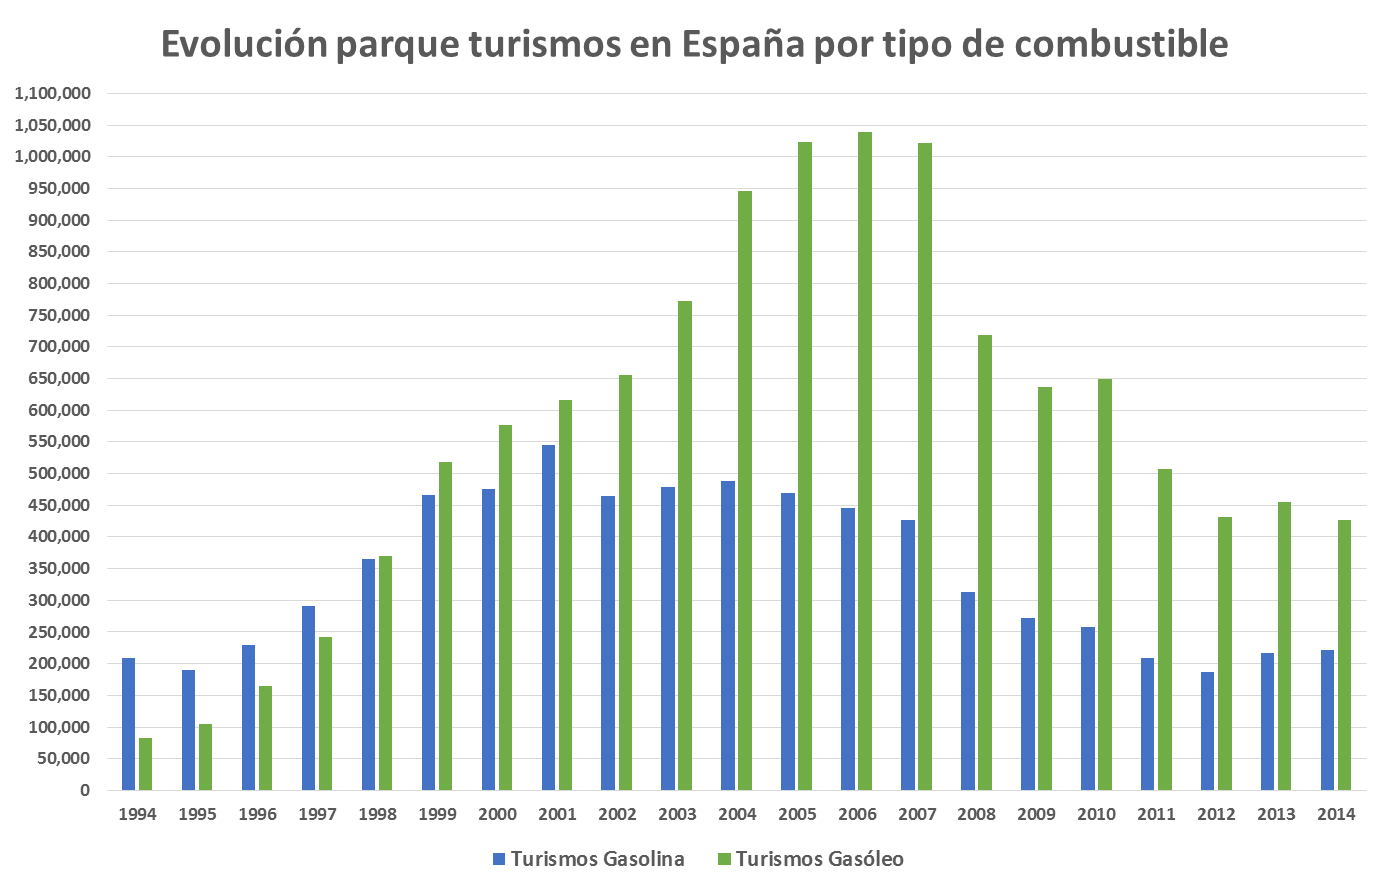
\includegraphics[width=0.6\textwidth]{Evolucionturismos.png}	 
	\caption[Evolución histórica de turismos diésel y gasolina en España]{Evolución parque turismos en España desde 1984 por motorización.\\ \textbf{Fuente:} \href{https://sedeapl.dgt.gob.es/IEST2/menu.do?path=/vehiculos/parque/&file=inebase&type=pcaxis&L=0&js=1}{Portal estadístico de la DGT}}	
\end{figure} \label{fig:EvolucionParqueTurismos}

\par Actualmente la protección del medio ambiente constituye una prioridad ineludible, particularmente en los países avanzados, aunque se ha extendido a la mayoría del resto de países con el Protocolo de Kyoto (1997) y con las cumbres mundiales de Clima, la última de las cuales se celebró en Nueva York (2014). Esta protección del medio ambiente se ha implementado mediante políticas ambientales que cada vez hacen las legislaciones más estrictas. En Europa actualmente están vigentes la Directiva 98/69/CE y la Directiva 2002/80/CE. En estas Normativas se establecen los valores límites para los motores de encendido por compresión ligeros. De las restricciones para los pesados se encarga la Directiva 2001/27/CE. Todas estas directivas establecen límites en términos de masa de partículas emitidas por kilómetro o por kWh.

\par Debido a esto, la mayoría de los estudios sobre emisiones de \index{partículas} partículas analizan exclusivamente los resultados de emisiones en masa. Sin embargo, también la \index{morfología} morfología de las partículas tiene gran importancia dada la notable influencia que ésta tiene sobre la salud humana y sobre el medio ambiente. Por tanto, además de regularse la masa de partículas emitida podría justificarse también algún tipo de regulación sobre el tamaño y la morfología de éstas. En concreto, la legislación medioambiental no es ajena a las normativas sobre el tamaño de las partículas y no es aventurado esperar que en el futuro alguna limitación del tamaño de las partículas se aplique también a las emisiones diésel. Más lejano aún y complejo resulta suponer, de momento, que otros aspectos de la morfología de las partículas puedan llegar a regularse.

\par Por otra parte, antes de ser expulsadas a la atmósfera, la morfología de las partículas tiene también un importante efecto sobre la eficiencia de retención de las \index{trampas de partículas} trampas de partículas, consideradas actualmente como uno de los sistemas de postratamiento necesarios en algunas estrategias de reducción de emisiones más interesantes de cara a cumplir las normativas de emisiones de los motores diésel.

\par Son precisamente los importantes efectos sobre la morfología de las partículas emitidas sobre los filtros de partículas, sobre la salud humana, sobre el medio ambiente y sobre el clima, los que justifican la realización de esta Tesis Doctoral, en línea con el creciente interés científico, como se demuestra en el estudio bibliométrico presentado en el apartado \ref{sec:Bibliometria}.

\section{Objetivos}\label{sec:Objetivos}

\par Principalmente, esta Tesis Doctoral se centra en tres objetivos, que son:

\begin{itemize}
	
	\item Estudio de cómo afecta la no esfericidad de la morfología de las partículas primarias a las características geométricas de los aglomerados diésel. En casi la totalidad de la literatura existente, se parte de la base de que los aglomerados están compuestos por partículas esféricas. Los efectos que pueden llevar a que las partículas no sean perfectamente esféricos son variados y pueden modelarse mediante un parámetro geométrico que permita determinar en qué cuantía la desviación de la idealidad esférica modifica los valores de la geometría fractal. Existen trabajos donde se han modelado estas geometrías, pero la manera en que afectan al prefactor y a la dimensión fractal está menos estudiado. Estos parámetros serán definidos en el capítulo \ref{cap:MetodosAnalisisFractal}. Partiendo de figuras que permiten imponer condiciones de contorno conocidas para dichos parámetros, es posible estudiar cómo se comportan éstos cuando la geometría de las partículas primarias se desvía de la esfericidad.
	
	\item Como se ha comentado anteriormente, para estudiar la geometría fractal de los aglomerados se han de asumir una serie de hipótesis que son aceptadas ampliamente en el ámbito de las emisiones de partículas diésel. Sin embargo, existen muy pocas referencias que cuestionen la validez de dichas hipótesis, o al menos, el rango de valores para los cuales su aplicabilidad está fuera de duda. Esta Tesis tiene como objetivo cuestionar algunas de estas hipótesis, entre ellas la hipótesis del número mínimo de partículas primarias para el cual un aglomerado puede ser considerado fractal o cuasi-fractal.
	
	\item Los fractales, como se expondrá a lo largo del Capítulo \ref{cap:MetodosAnalisisFractal} se encuentran en la naturaleza y es el lenguaje geométrico natural. Parece lógico que una metodología de análisis fractal aplicada al campo de emisiones pueda usarse sin muchas modificaciones a otros campos. Como ejemplo de ello, se aplicarán algunas técnicas a la caracterización fractal de rocas y fracturas hidráulicas usadas para la explotación de hidrocarburos.
	
	\item Con objeto de poder analizar una gran cantidad de parámetros y de morfologías para su posterior comparación, es necesario disponer de herramientas informáticas flexibles y desarrolladas \textit{ad hoc} para las aplicaciones objeto de interés de esta Tesis. Por ello, otro objetivo, aunque menor, de esta Tesis es la mejora y desarrollo de aplicaciones donde se implementen las metodologías desarrolladas en esta Tesis.
	
\end{itemize}

\par Para la consecución del primer objetivo se ha partido del enfoque geométrico seguido en la Tesis de Francisco Martos \cite{martosphD:2006} y en \cite{lapuertaetal:2006,lapuertaetal:2010}. A través de figuras geométricas cuya dimensión fractal es impuesta se pueden determinar el modelo matemático que siguen los parámetros a estudio y ver la influencia de la hipótesis de no esfericidad en la morfología de las partículas diésel. Para un estudio más pormenorizado se utilizó la herramienta informática que de desarrolló en el Proyecto Fin de Carrera \cite{vieraPFC:2014}. El uso de herramientas informáticas es de vital importancia para el estudio de la geometría de aglomerados bajo ciertas condiciones.

\par De igual modo, mediante el uso de otra herramienta informática \cite{delblancoPFC:2015} se puede analizar la dependencia de los resultados con respecto a una de las hipótesis impuestas en los modelos geométricos. Los aglomerados de partículas diésel son asimilados a figuras fractales cuando el número de partículas primarias es superior a cierto número, habiendo un consenso establecido para dicho número, pero sin una justificación lo suficientemente elaborada. La validez en el campo de las partículas diésel, donde los aglomerados tienen usualmente menos de doscientas ($n_{po}\,<\,200$) fue demostrado por \cite{megaridisetal:1990}. Después ha sido utilizado por numerosos autores para la caracterización de hollín \cite{zhuetal:2003,leeetal:2002,caietal:1995,gorbunovetal:1999,zuritaetal:2002,parketal:2004}.

\par El disponer de una metodología que sólo depende de la geometría y no del proceso que da origen a esa morfología, permite que las técnicas y herramientas desarrolladas en la presente Tesis puedan aplicarse a cualquier campo donde la naturaleza fractal de los fenómenos sea relevante.

\section{Antecedentes}\label{sec:Antecedentes}

\par El Grupo de Combustibles y Motores lleva estudiando las emisiones de los Motores diésel durante más de veinte años. Sus esfuerzos se han centrado en la caracterización de combustibles, tanto convencionales como alternativos. Cuando aún la tecnología de motores de encendido por compresión no había superado a la tecnología de los motores de encendido provocado, aunque estaba cerca de lograr este último hito, se presentó la Tesis de Rosario Ballesteros Yáñez \cite{chariphD:2002}. El trabajo de investigación que se presenta en su Tesis Doctoral se enmarca dentro del desarrollo y puesta a punto de herramientas de caracterización y análisis de partículas diésel. Además, los resultados experimentales obtenidos de ensayar combustibles de diferente origen y especificaciones permitieron mejorar el conocimiento que se poseía de los procesos que tienen lugar en el motor y que contribuyen a la generación y emisión de partículas diésel y ayudaron a establecer las directrices en cuanto a búsquedas de posibles nuevos combustibles de automoción y de soluciones óptimas en las que las prestaciones y las emisiones de los motores permaneciesen dentro de unos niveles adecuados. Este trabajo fue el primer estudio que se realizó sobre combustibles y emisiones de partículas diésel dentro de este grupo de investigación y constituyó un antecedente directo de otras Tesis Doctorales. 

\par Tal fue el caso de la Tesis de Francisco Javier Martos Ramos \cite{martosphD:2006}. Fue el primer trabajo dirigido hacia la caracterización morfológica de partículas mediante técnicas fractales. Se propone un método teórico-experimental para determinar los parámetros característicos, desde el punto de vista de la geometría fractal, de las emisiones provenientes de los motores diésel. Como continuación a esta Tesis Doctoral, José Martín Herreros Arellano \cite{martinphD:2009} centró su Tesis en estudiar el efecto del modo de funcionamiento y del combustible en la morfología de las partículas diésel. A partir de micrografías donde se estimaban el radio de giro y él área proyectada, se determinaban parámetros morfológicos de las partículas. Desde el punto de vista de emisiones, existen diferentes estrategias en cuanto a carga y regeneración de trampas de partículas. En este contexto, la Tesis de Fermín Olivas Miñana \cite{ferminphD:2012} se centró en caracterizar la influencia del combustible y de distintas condiciones operativas sobre el tamaño de las partículas, ampliando el estudio presentado en el artículo \cite{lapuertaetal:2007}.

\par Adicionalmente a estas Tesis, cabe mencionar el Proyecto Final de Carrera de Enrique Viera Luis \cite{vieraPFC:2014} que consistió en la implementación de una herramienta informática incluyendo el modelo propuesto en la Tesis de Francisco Javier Martos Ramos \cite{martosphD:2006}, ampliado en los artículos \cite{lapuertaetal:2010} y complementados por el Proyecto Final de Máster de Juan José Expósito González \cite{expositoPFM:2012}, corrigiendo algunas erratas en las ecuaciones de éste último. 

\par Los modelos empleados tienen hipótesis subyacentes que necesitan de herramientas matemáticas para su validación o para la limitación del rango de validez. En este sentido, el Trabajo Final de Grado de Marcos del Blanco Adán \cite{delblancoPFC:2015} desarrolla una metodología computacional ampliamente reconocida y aceptada en el campo de la geometría fractal.
\par El encuadre de la presente Tesis con referencia a los trabajos citados anteriomente se pueden ver en la Tabla.

\section{Metodología}\label{sec:Metodologia}

\par La metodología seguida en esta Tesis tiene un carácter eminentemente teórico. A partir de planteamientos matemáticos no excesivamente complejos se pretende ahondar en el conocimiento de aspectos morfológicos de agregados. Sin embargo, debido a que de abordan temas reales, no se descuida la aplicabilidad práctica de los resultados obtenidos. De igual forma se intentar maximizar las sinergias entre la práctica con la teoría, mediante las bases de datos de imágenes acumuladas desde hace años en el Grupo de Combustibles y Motores de la Universidad de Castilla-La Mancha.

\par La mayor parte de los ensayos se llevaron a cabo en las instalaciones de motores existentes en las Universidades de Castilla-La Mancha y de Málaga. Por un lado, en las primeras hay preparados para diferentes ensayos motores típicos de automoción de inyección directa completamente instrumentados con el triple objetivo de realizar medidas precisas, mantener el control de la instalación y asegurar la repetitividad de las condiciones de ensayo. En etas instalaciones experimentales hay disponibles técnicas experimentales de cierta complejidad que permiten la validación en tendencias de algunos resultados de los modelos planteados, así como otras técnicas experimentales menos complejas cuyos resultados alimentan a los modelos propuestos. Por otro lado, en las últimas hay disponibles técnicas experimentales correspondientes a la visualización de las partículas diésel y su posterior tratamiento digital. Los resultados de estas técnicas son de tipo geométrico y sus resultados son fundamentales para la entrada al modelo planteado sobre la morfología de partículas.

\par Con anterioridad e independencia a esta Tesis se obtuvieron una gran multitud de imágenes de aglomerados. Mediante técnicas de tratamiento de imágenes se pueden tratar para obtener parámetros geométricos característicos y usarlos para alimentar los modelos matemáticos de obtención de propiedades geométricas. Las interconexiones entre los métodos experimentales y teóricos se han esquematizado en la Figura.

\par La incorporación de técnicas de análisis de imágenes de tipo fractal ha permitido calcular la dimensión fractal de aglomerados de geometría conocida. Tal es el caso del método de Box-Counting que se explicará detalladamente en el Capítulo \ref{cap:MetodosAnalisisFractal}. Éste, junto con el resto de técnicas propuestas componen el conjunto de herramientas informáticas utilizadas.

\section{Bibliometría}\label{sec:Bibliometria}

\par Con el fin de demostrar la actualidad del interés de esta Tesis, se han realizado dos estudios bibliométricos, que se detallan en las Figuras y . Estos estudios bibliométricos se han realizado con el \emph{ISI Web of Knowledge} que tiene en su base de datos todas las publicaciones de interés internacional desde 1945.

\section{Viabilidad}\label{sec:Viabilidad}

\section{Desarrollo del Documento de la Tesis}\label{sec:DesarrolloDocumento}

\par La memoria de la presente Tesis Doctoral se compone de un total de nueve capítulos. En el primero de ellos se introduce y se justifica el porqué de la realización de este documento. Se hace una breve descripción de la historia y situación actual del grupo de investigación y se encuadra la Tesis Doctoral dentro de la línea de investigación. Igualmente, se expone la metodología seguida para la realización de la Tesis.

\par El segundo contiene una revisión del estado del arte en la morfología de las partículas en general, y específicamente sobre las partículas diésel. Inicialmente se hace una pequeña revisión a los distintos fenómenos de transporte a los que se pueden ver sometidas las partículas diésel, y que pueden dar lugar a distintos tipos de uniones. Una vez analizado cómo se conforman las partículas diésel desde su nucleación se comentan las distintas maneras de definir el tamaño de éstas y las funciones de distribución típicas. Posteriormente se describen los parámetros utilizados para definir las características morfológicas de las partículas. Se sigue con una descripción de geometrías fractales de campos distintos al de emisión de partículas en procesos de combustión. Finalmente, se comentan las implicaciones de la morfología y el tamaño de las partículas diésel sobre el medio ambiente y sobre la salud pública.

\par Dada la creciente importancia de los fractales en diversas aplicaciones, el capítulo tercero se centra en los métodos de análisis fractal desde un punto de vista puramente teórico. Se dan ejemplos de fractales conocidos y se hace un recorrido por esta incipiente rama de las matemáticas moderna, con reseñas históricas sobre sus principales contribuyentes. De carácter eminentemente teórico, es el capítulo más general de esta Tesis, aunque incluye aplicaciones a diversas ramas de la ingeniería. Una de ellas, las partículas diésel ocupa un apartado dentro de este capítulo. Se sigue con una descripción de otros fenómenos caracterizados por la geometría fractal, como son la caracterización de rocas y de dinámica de fluidos en medios porosos. Finalmente, se tocan otros temas adyacentes y que pretenden despertar la curiosidad de la aplicabilidad de las técnicas fractales como son el análisis de mercados y otras ramas del saber.

\par El cuarto capítulo es una particularización del tercero, centrándose en las partículas diésel. Se comienza dando unos conceptos básicos sobre los métodos geométricos de caracterización de partículas diésel mediante geometría fractal. Estos métodos se centran en la situación ideal de contacto puntual entre partículas. Posteriormente se describe el modelo empleado, desarrollando las ecuaciones matemáticas para los casos estudiados.

\par El quinto capítulo parte del modelo desarrollado en el capítulo anterior, relajando una de las hipótesis empleadas hasta ese capítulo. Se parte de partículas no esféricas, sino que están aplastadas. Primero se describen los procesos por los cuales la geometría de una partícula primaria podría no ser esférica. Después se define el parámetro físico para modelar esta geometría. Por último, se desarrollan las ecuaciones correspondientes y se compara con los resultados obtenidos en el capítulo cuarto.

\par En el sexto capítulo se realiza una crítica de las hipótesis del modelo. Se pretende comprobar la robustez de dichas hipótesis empleando diferentes herramientas matemáticas. Primero se introduce el método del Box-Counting que no depende de la geometría subyacente al problema. Se describe en qué consiste dicho modelo en primer lugar. Después, se aplica a figuras conocidas. Esto es necesario para comprobar la validez de este método. Dos hipótesis se ponen a prueba: la primera, la monodispersidad, es decir, la uniformidad en el tamaño de las partículas primarias que componen el aglomerado. La segunda y última, la esfericidad.

\par Como se ha comentado anteriormente, se dispone de una amplia base de datos con imágenes de aglomerados obtenidos en motores diésel, bien con combustible convencional o biocombustibles. Utilizando las herramientas presentadas en los capítulos anteriores, se pretende caracterizar la "huella" fractal de cada combustible. Para ello, los parámetros geométricos característicos juegan un papel determinante, como se verá en el Capítulo \ref{cap:AplicacionModelo}.

\par La Tesis termina con las conclusiones que se extraen a partir del trabajo realizado y sugerencias de trabajos futuros que se puedan derivar de lo desarrollado en esta Tesis.

\section{Resumen del Capítulo}\label{sec:ResumenCapitulo1}

\newpage
\bibliographystyle{Config/ealpha}	
\bibliography{Chapters/Bibliografia}
		\input{Chapters/02ProcesosFormacionYMorfologia.tex}
		\pagestyle{plain}
\chapter{INSTALACIONES EXPERIMENTALES}\label{cap:InstalacionesExperimentales}
\vspace{0.2cm}
\noindent\rule{\linewidth}{1.5pt}\\
\startcontents[chapters]
\printcontents[chapters]{}{1}{}
\vspace{0.2cm}
\noindent\rule{\linewidth}{1.3pt}\\
%\dominitoc
\newpage

\newpage
\bibliographystyle{Config/ealpha}		
\bibliography{Chapters/Bibliografia}

		\pagestyle{plain}
\chapter{MÉTODO DE ANÁLISIS FRACTAL PROPUESTO}\label{cap:MetodosAnalisisFractal}
\vspace{0.2cm}
\rule{\linewidth}{1.5pt}\\
\startcontents[chapters]
\printcontents[chapters]{}{1}{}
\vspace{0.2cm}
\rule{\linewidth}{1.5pt}\\
%\dominitoc
\newpage
\section{Conceptos básicos}\label{sec:ConceptosBasicos}
\par Las partículas emitidas en procesos de combustión, bien sean en llamas en hornos, quemadores o en motores diésel, forman conjuntos de partículas llamados \index{aglomerados} \emph{aglomerados}. Cada partícula constituyente de dicho aglomerado se denomina \index{partícula primaria} \emph{partícula primaria}. Asimismo, los aglomerados formados en las tecnologías que involucran suspensiones sólidas coloidales están formados a menudo por partículas primarias \index{monómeros}(\emph{monómeros}) con formas parecidas a \index{esférulas} \emph{esférulas}, cuyos diámetros son muy uniformes en tamaño. Algunos procesos de formación de partículas tienen como resultado final la obtención de productos diferentes a los de partida. Tal es el caso de la industria de los pigmentos. Mientras, otros procesos generan subproductos, siendo la formación de hollín en el conducto de escape de un motor Diésel un ejemplo de estos últimos. Aunque los procesos de formación puedan ser muy diferentes, la formación de partículas de SiO$_2$ y TiO$_2$ llevan a la formación de partículas cuya apariencia física es muy parecida. Estos son sólo dos ejemplos de una amplia variedad de entornos industriales cuyos procesos conllevan la formación de aglomerados con morfologías que no sólo son similares, sino que también sus propiedades son muy similares las unas de las otras, con independencia del material de entrada al proceso. Las propiedades resultantes dependen fuertemente de la disposición espacial y la morfología, la cual tiene un fuerte impacto en las propiedades finales de los aglomerados.

\par El último es el caso de los aglomerados de hollín diesel, entre otros \cite{lapuertaetal:2007}. En los estudios de simulación, es común asumir un diámetro uniforme para las partículas primarias, \cite{wuetal:1993,tandonetal:1995,ohetal:1997,leeetal:2002,zhuetal:2003}, ya que se ha probado que la polidispersidad no afecta significativamente a los parámetros morfológicos que describen el aglomerado \cite{busheletal:1998}. Estas partículas primarias se disponen en el aglomerado formando racimos irregulares con tamaños, formas y masas diferentes los unos de los otros. Pueden considerarse como estructuras cuasifractales y se acepta que, en el caso de estar compuestos por un número suficiente de partículas primarias pueden describirse mediante la \emph{Ley de Potencias}, siendo la \textbf{dimensión fractal} y el \textbf{prefactor} como los parámetros característicos \cite{bonczyketal:1991}. Los tamaños tan dispersos de los aglomerados, junto con los bien conocidos efectos medioambientales y sobre la salud que tiene la morfología de los aglomerados (no sólo con respecto al tamaño sino también con respecto a la forma) \cite{kittleson:1998,meakinetal:1989} hacen necesaria una descripción cuantitativa adecuada de los aglomerados de hollín.

\par La forma más común de cuantificar esta irregularidad es usando la dimensión fractal, adoptada de \cite{mandelbrot:1983} partiendo de la propuesta previa de Félix Hausdorff. La aplicación de una dimensión fractal a los aglomerados de hollín diésel supone asumir que estos aglomerados se corresponden con geometrías fractales. Aunque los aglomerados de hollín se pueden clasificar como racimos granulosos o granulares siguiendo la concepción original de Mandelbrot, se consideran usualmente estructuras cuasifractales, ya que no pueden ser ciertamente ser autosimilares (o autoescalares como las denominó Mandelbrot) a menos que estén compuestas de un número muy grande de partículas primarias.

\par En la literatura se han propuesto diferentes métodos experimentales para determinar la dimensión fractal de aglomerados de hollín a partir de sus imágenes planas obtenidas mediante \textit{Microscopio de Transmisión Electrónica} (TEM por sus siglas en inglés). El más común se basa en ajuste lineal del diámetro de giro frente al número de partículas primarias, en un diagrama log-log \cite{leeetal:2002}

\begin{equation}
\ln(n_{p_o})\,=\,\ln(k_{f})+D_{f}\ln(\frac{d_{g}}{d_{p_o}})
\label{eq:leydepotencias}
\end{equation}

\par Este método se deriva de la aplicación de la \index{Ley de Potencias}, la cual está considerada ampliamente como la ecuación característica que gobierna las estructuras fractales o cuasifractales \cite{samsometal:1987,caietal:1995,koyluetal:1995}, etc. La dimensión fractal \nomenclature{$D_{f}$}{Dimension Fractal} se obtiene entonces como la pendiente de la recta de regresión, mientras que el prefactor \nomenclature{$k_{f}$}{Prefactor de la Ley de Potencias} se identifica con el valor cuya abscisa es cero. Sin embargo, este método tiene cinco desventajas importantes:

\begin{enumerate}
\item Es incapaz de dar una dimensión fractal y un prefactor para los aglomerados de forma individual. En cambio, da un valor medio de ambos parámetros para una población grande de aglomerados. Una descripción individual de la morfología del aglomerado abría las posibilidades de una mejor discriminación de los efectos de las condiciones operativas del motor, tipo de combustible utilizado, condiciones térmicas en el conducto de escape, etc. sobre el tamaño, forma y efectos potenciales medioambientales de las emisiones de hollín. Pocos métodos geométricos se han propuesto para la determinación individual de la dimensión fractal de aglomerados de hollín hasta la fecha \cite{lattuadaetal:2003,lapuertaetal:2006,wozniaketal:2012}.
\item El número de partículas primarias que componen el aglomerado es desconocido, y se estima normalmente a través de otra Ley de Potencias distinta que intenta reproducir el solape entre partículas primarias cuando el aglomerado se proyecta en un plano, \cite{medaliaetal:1969,megaridisetal:1990}, \cite{brasiletal:1999,leeetal:2003}. Sin embargo, el exponente para esta Ley de Potencias adicional, $z$, no se determina de forma unívoca, ya que de hecho depende de la forma y tamaño del aglomerado \cite{ohetal:1997}. El solape y el aplastamiento no deben confundirse: el primero es un efecto visual de las partículas ocultas tras otras partículas en la proyección plana, mientras que el último es un efecto morfológico debido a la colisión de partículas primarias que resulta en geometrías que están lejos de ser esféricas.

\begin{equation}
\ln(n_{p_o})\,=\,\ln(z)+\ln(\frac{A_{p}}{A_{p_o}})
\label{eq:leydepotenciassolape}
\end{equation}

\item El diámetro de giro del aglomerado se identifica normalmente con el diámetro de giro de su proyección plana \cite{rogaketal:1992,koyluetal:1995,ohetal:1997}, a pesar de que se ha probado que subestima el diámetro de giro del aglomerado tridimensional. Este error lleva a que los métodos basados en proyecciones de imágenes planas subestimen la dimensión fractal de las estructuras tridimensionales \cite{rogaketal:1992,nelsonetal:1990,adachieetal:2007}.

\item Se supone tamaño uniforme para las partículas primarias. Esta suposición podría parecer muy restrictiva. De hecho, se puede probar que se puede obtener una distribución de tamaños estadística en todos los procesos que involucran interacción de partículas \cite{busheletal:1998}. Sin embargo, el asumir tamaño uniforme para modelar la morfología de los aglomerados constituidos por partículas primarias ha demostrado ser un enfoque correcto al problema.

\item Las partículas primarias se asumen esféricas, sin tener en cuenta los efectos de aplastamiento, que podrían afectar al prefactor y a la dimensión fractal obtenidos \cite{ohetal:1997,brasiletal:1999,alzaitoneetal:2009}.
\end{enumerate}

\par La investigación doctoral que se desarrollará comienza desde la base del modelo propuesto por \cite{lapuertaetal:2006} e intenta resolver los inconvenientes 2 a 4 anteriormente mencionados. La primera parte de esta investigación se dedica al análisis fractal  basada no solamente en la forma de los aglomerados a partir de sus proyecciones planas, sino también a partir de su opacidad. La \emph{Ley de Beer-Lambert}, que proporciona la transmitancia lumínica de imágenes de sólidos en escala de grises, se uso como base para determinar el número de partículas primarias ocultas detrás de las visibles. A partir del número de partículas primarias de cada aglomerado individual, su masa, momento de inercia, diámetro de giro se determinaron su densidad aparente y su dimensión fractal sin hipótesis adicionales acerca del solape y sin extrapolación de patrones promedio. Esta metodología ha sido publicada en la revista \textit{Measurement Science and Technology} y se encuentra en el Apéndice \ref{app:BeerLambert} al final de esta tesis.

\section{Descripción del modelo geométrico}
\section{Algoritmo del modelo}
\section{Hipótesis del modelo}


\newpage
\bibliographystyle{Config/ealpha}		
\bibliography{Chapters/Bibliografia}
		%\chapter{GENERALIZACIÓN A PARTÍCULAS DEFORMADAS}
%\startcontents[chapters]
%\printcontents[chapters]{}{1}{}
\newpage
\section{Modelado del prefactor $k_f$}
\section{Coeficiente de solape para partículas deformadas $z$}

\newpage
%\bibliographystyle{plain}
\bibliographystyle{Config/ealpha}
% \bibliographystyle{apalike}
% \bibliographystyle{aea}
\bibliography{Chapters/Bibliografia}
%\putbib{Tesis}
		%\chapter{APLICACI�N DEL MODELO}
\minitoc


%\pagebreak
\bibliographystyle{eunsrt}
\bibliography{Tesis}
%\putbib{Tesis}
		
	\backmatter
	
		\appendix
		%
		% CONFIG. TODO
		%
		\pagestyle{plain}
\chapter{Apéndice: Beer-Lambert}\label{app:BeerLambert}
\vspace{0.2cm}
\rule{\linewidth}{1.5pt}\\
\startcontents[chapters]
\printcontents[chapters]{}{1}{}
\vspace{0.2cm}
\rule{\linewidth}{1.5pt}\\
%\dominitoc
\newpage
		\chapter{Teor�a sobre polinomios factoriales}\label{app:ApendiceII}
\startcontents[chapters]
\printcontents[chapters]{}{1}{}
\newpage


		\newpage{\pagestyle{empty}\cleardoublepage}
		\pagestyle{empty}
		\printindex		
		
	\end{onehalfspace}
\end{document}